\documentclass{article} % For LaTeX2e
\usepackage{Asst-1-Ye,times}
\usepackage{hyperref}
\usepackage{url}
\usepackage{lipsum}
\usepackage{float}
\usepackage{listings}
\usepackage[pdftex]{graphicx} 


\title{CSE597 Homework1 Report: Low Dimension Vector Representation of Synonymy}


\author{
Jiarong Ye\\
Department of Computer Science and Engineering\\
\texttt{jxy225@psu.edu} \\
}



\newcommand{\fix}{\marginpar{FIX}}
\newcommand{\new}{\marginpar{NEW}}

\nipsfinalcopy % Uncomment for camera-ready version

\begin{document}


\maketitle

\section{Introduction}


\begin{itemize}
	\item First, in order to obtain seed words, I generate nouns and verbs from the Brown Corpus \cite{francis1979brown} using the python NLTK\cite{Bird:2006:NNL:1225403.1225421} package. In this process, the way I implemented in the assignment is slightly different from the instruction. The approach suggested is to choose one random number generator and generate 10 nouns and 10 verbs ready for the synonyms lists construction. However, since the method I applied for synonyms extraction is by coding it up with the Synset in WordNet of NLTK package, among most cases, I was not able to extract 4 synonyms of some words among the 20. Thus, regarding the synonyms extraction approach I used, initial 10 nouns and verbs was not enough. Therefore, I adopted another approach as follows:
	\begin{itemize}
		\item[*] extract all words from Brown Corpus
		\item[*] filter nouns whose POS tag is \textbf{NN} and verbs whose POS tag is \textbf{VB}
		\item[*] shuffle the noun and verb list using \textbf{numpy.random.shuffle}
		\item[*] from these two lists, select words in order (since they are already shuffled, it would be equivalent to random selection), extract the words with more than 4 synonyms, and repeat until there are 5 synonym lists for nouns, with 5 words in each list, and same for verbs, then stop and break out the loop
	\end{itemize}
	randomly gathered words list:
	\begin{itemize}
		\item nouns:\\
		1. tendency, inclination, leaning, propensity, trend\\
		2. person, somebody, someone, soul, individual\\
		3. volume, intensity, book, bulk, loudness\\
		4. statement, instruction, argument, affirmation, assertion\\
		5. instance, example, case, illustration, representative
		
		\item verbs: \\
		1. put, cast, couch, set, pose\\
		2. supply, furnish, append, cater, render\\
		3. take, shoot, carry, train, read\\
		4. commit, intrust, practice, place, devote\\
		5. identify, key, distinguish, discover, describe
	\end{itemize}


\end{itemize}


\begin{figure}[H]
	\centering
	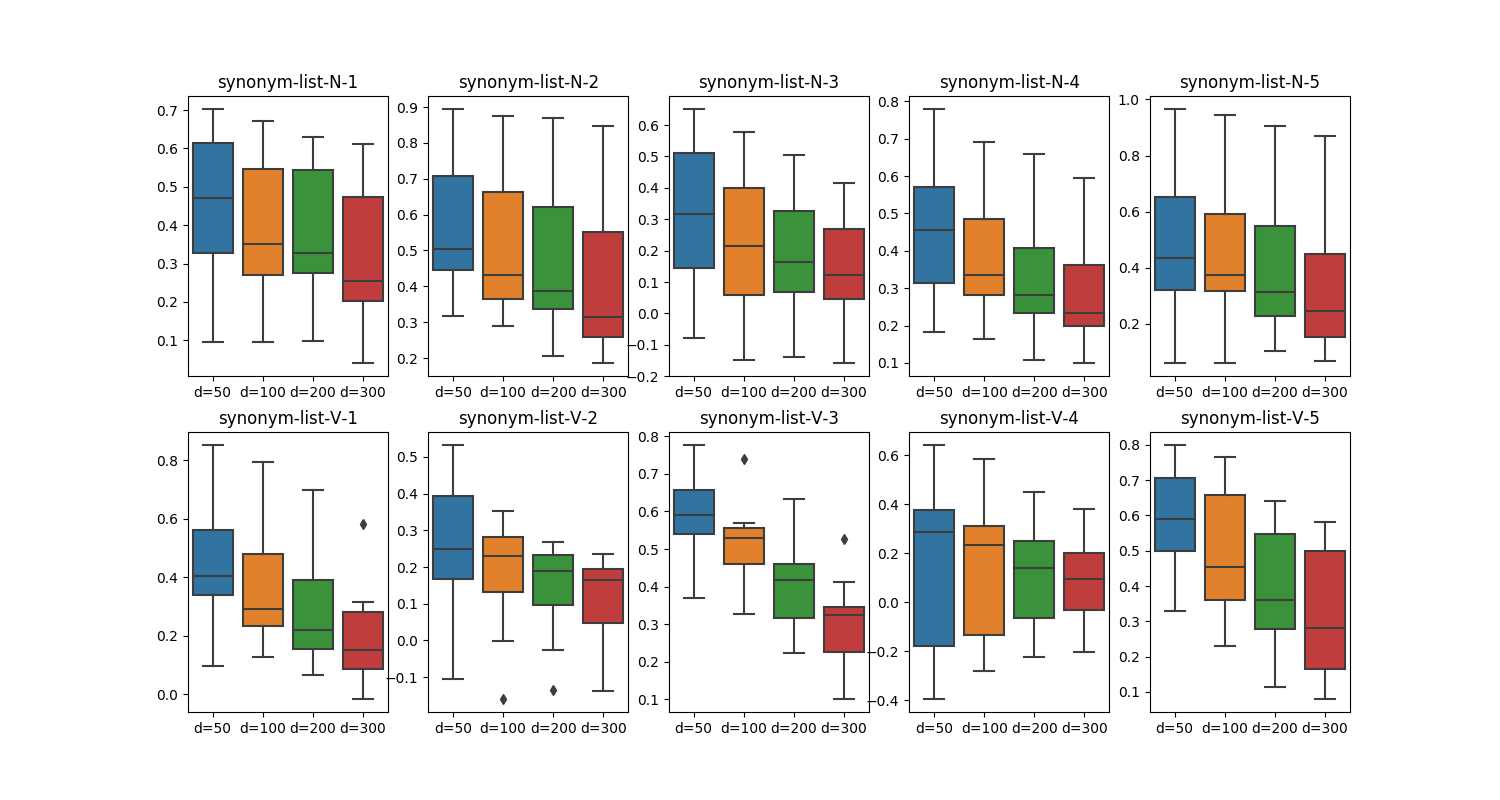
\includegraphics[width=0.9\linewidth]{../whiskerplot}
	\caption{sensitivity whisker plots of each noun and verb list}
	\label{fig:whiskerplot}
\end{figure}



\begin{figure}[H]
	\centering
	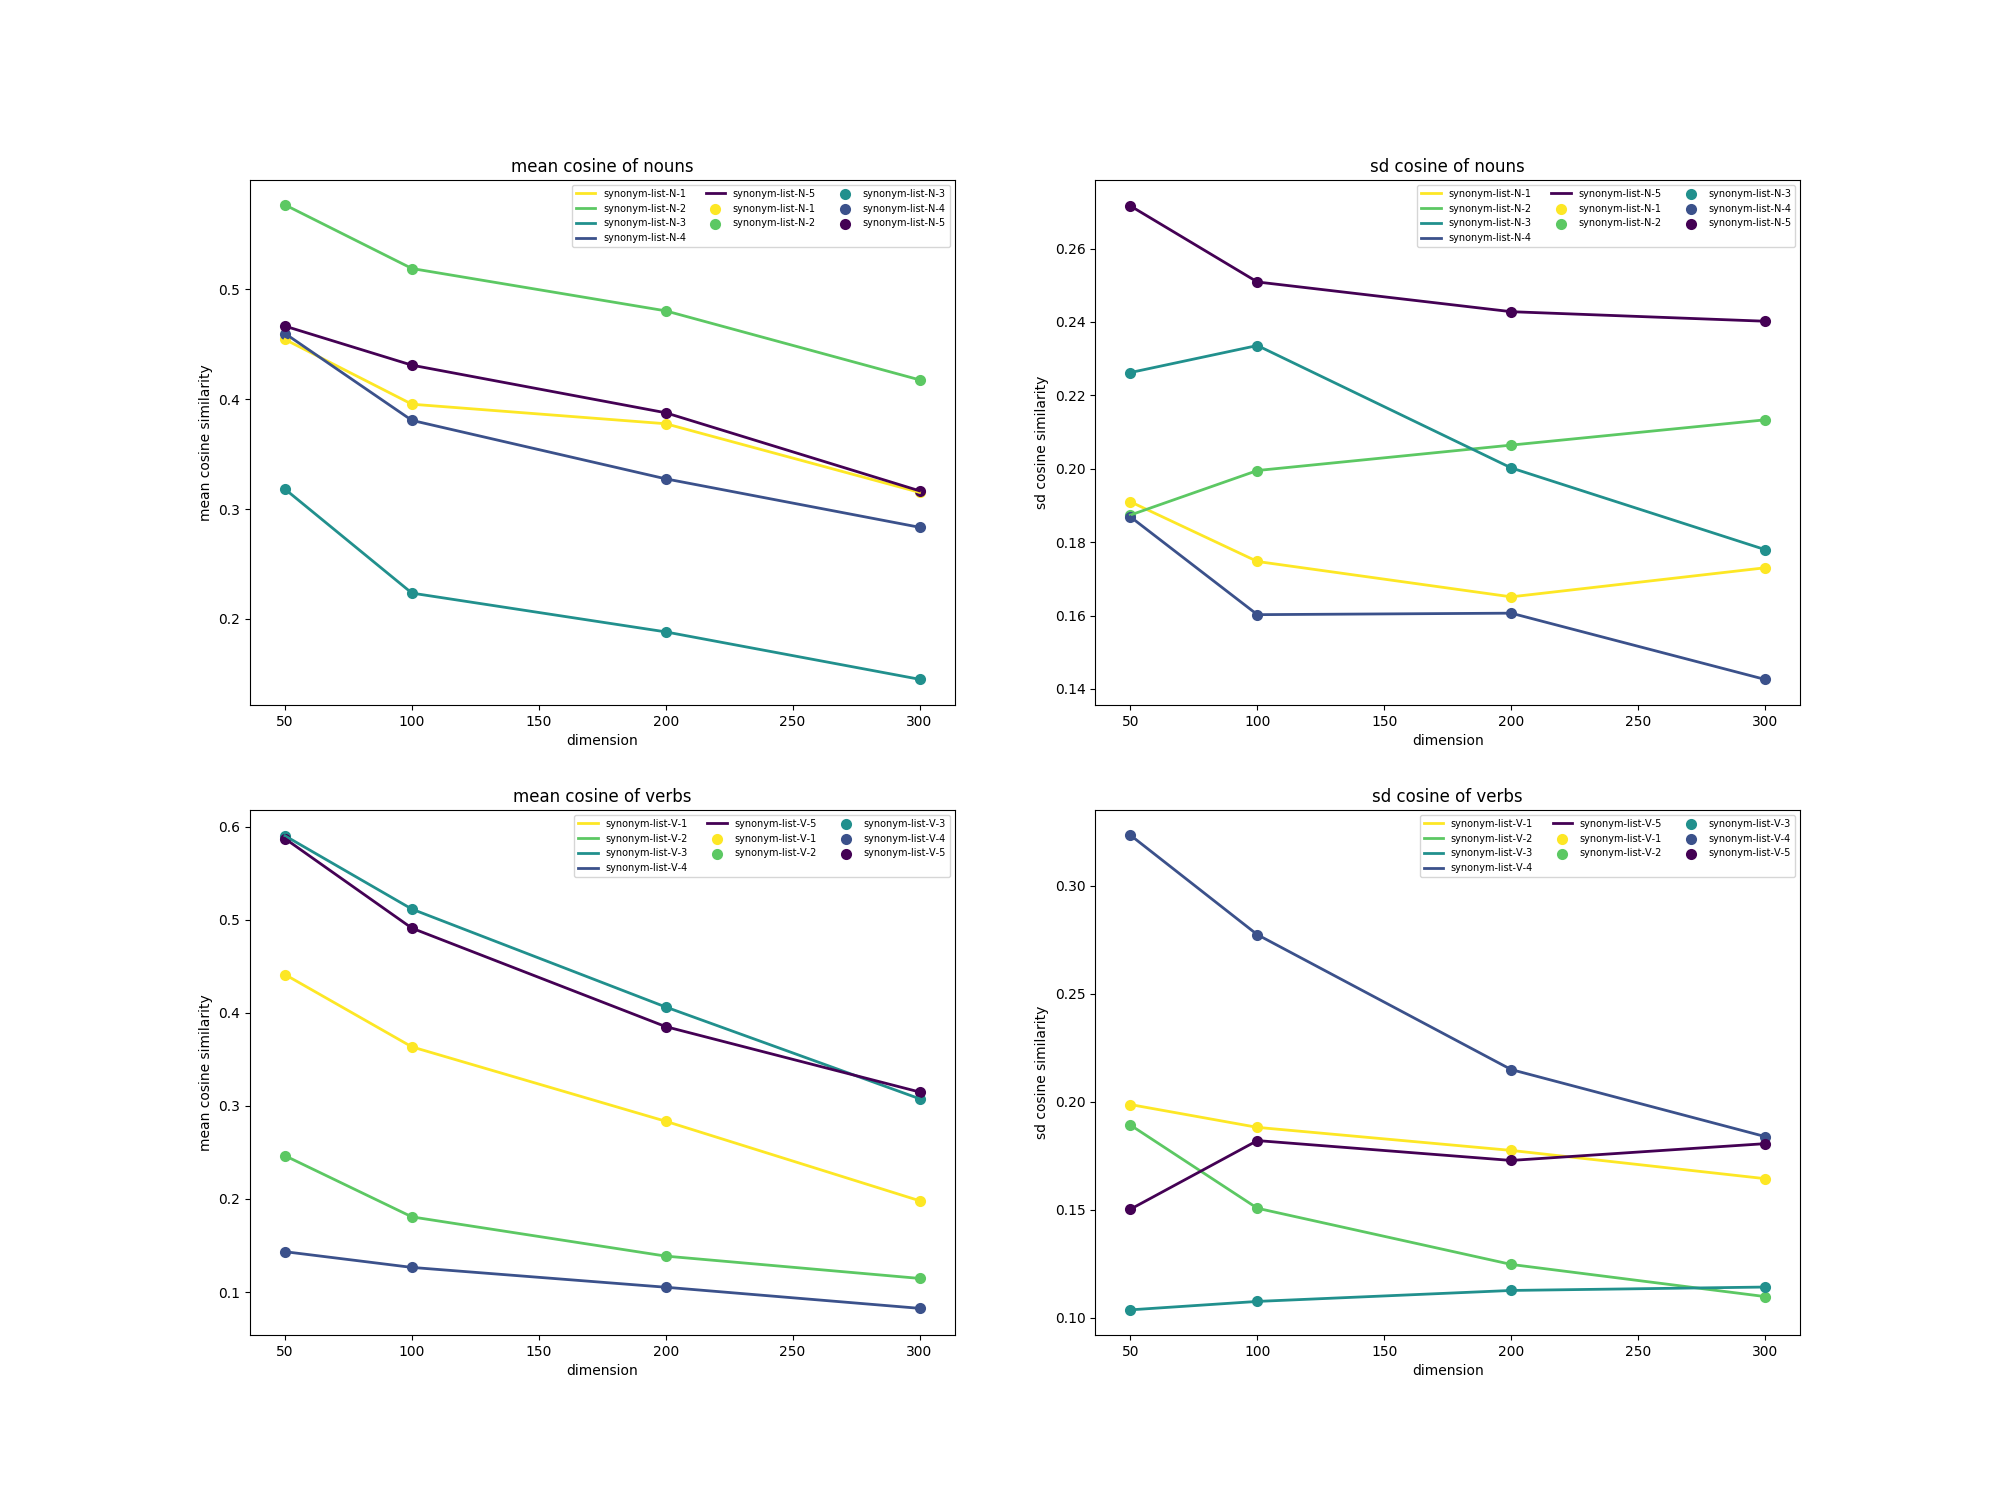
\includegraphics[width=1.1\linewidth]{../mean_sd}
	\caption{performance plots of nouns and verbs}
	\label{fig:meansd}
\end{figure}

	



\section{Conclusion}

\begin{itemize}
		
	\item The assignment recommend to select seed words from a dictionary or
	WordNet rather than from the GLoVE\cite{pennington2014glove} vocabulary for the reason that 
	the word list in GLoVE includes lots of words from specific domain, such as occupation titles, company names, names of specific locations, etc. 
	\begin{itemize}
		\item[*] For instance, I randomly (with \textbf{numpy.random.choice}) select 50 words from GLoVE words and the list returned are not optimal for a manual seed word extraction:\\
		
		\textit{'dagli' 'swarmer' 'eliciting' 'jabar' '57mm' 'certegy' '12n' '13:09'
			'bregier' 'desi' 'pretexts' 'gugelmin' 'wickstrom' '118-year' 'rackham'
			'soft-shelled' 'broker-dealer' 'bilmes' '2,728' 'capcities' 'renditions'
			'reboost' 'al-arsuzi' 'scis' 'higuain' 'caneira' 'ilyushin-76'
			'crownpoint' 'valeurs' 'purgatoire' 'akaba' '53.58' 'osnabrueck' 'jayme'
			'basketbol' 'nebeker' 'fightin' '0520' 'verrazano-narrows' 'moldovia'
			'lightyears' 'tinges' 'jingnan' 'drenner' 'm1903' 'carwood' 'slow-down'
			'peenemünde' 'rfb' '2,913'}\\
		
		So if using the GLoVE vocabulary as pool for seed word extraction, it would be more computationally expensive because most words in the list might not have more than 4 synonyms, so in order to get the synonyms list as required, more words need to be tested and filtered out, which would take more time. (However, for the words in GLoVE which meet the requirement for constructing synonyms lists, the result is actually quite similar compared with the outcome with seed words extracted from other vocabulary source.)
	\end{itemize} 
	
	
	
	\item Across all 5 noun synonym lists and 5 verb synonym lists, it's unlikely that a consistent pattern is present here. From the observation of Figure 2, the general trend of mean cos similarity is decreasing. In the standard deviation of cos similarity plot, the pattern does not appear to homogeneous. The trend is not monotonically increasing or decreasing, but with some fluctuations, especially with nouns. To conclude, the dimension with the highest mean cosine similarity (which is d=50) does not necessarily have the lowest standard deviation, the result heavily depends on the choice of seed words.\\
	
	The higher the dimension of word vectors get, the lower the mean cosine similarity is. So it is reasonable to draw the conclusion that if $d>300$, the results actually would not be better. But the trend of standard deviation does not share the same pattern. One possible reason for denying the existence of consistent pattern is as the dimension goes higher, the feature set is expanded, with more parameters, the risk of over-fitting increases as well, in which case the word embedding is more likely to be affected by noise, therefore explaining the fact that from what we observe in Figure 2, the standard deviations do not present a monotonical and consistent pattern.\\
	
	
	Another possible reason could be because the lower dimensional vectors such as 50d in this case, may contain primarily syntactic information, and higher dimensions such as 300d have more spaces that contain contextual information. So the reason why the mean cosine similarity decreases when dimension goes up could be the simplicity of word similarity task itself. Applying cosine distance to calculate the similarity of two words does not require much deep contextual and topical information of the word, thus it's reasonable that in a very high dimensional space, the cosine distance of two synonyms might be far.\\
	 
	
	Therefore, the concept of the best dimension should be dependent on specific tasks, in this task of word similarity calculation, the word vector of lower dimension works better, but in another task, say, topic modeling, that might be where high dimensional word vectors excel. 
	
	
	
	\item From the sensitivity plot, each synonym list does not appear to have much individual variation in mean/sd cosine similarities. The mean cosine similarity is decreasing in all synonym lists, the lowest dimension has the highest mean cosine but with different slope. And the pattern for range and standard deviation is unclear and not consistent for each list, so it would probably be better to conclude that the mean and its sd vary independently. In the particular set of words chosen for this experiment, there are no outliers in all the synonym lists of nouns, however, outliers do present in 3 out of 5 synonym lists of verbs: there is one in the first synonym lists of verbs at $d=300$, there are two in the second synonym lists of verbs at $d=100, d=200$, there are also two in the third synonym lists of verbs at $d=100, d=300$.
	
	
	\item From the sensitivity and performance plots, we could see the mean cosine similarity is generally decreasing, both for nouns and verbs, but the range appears to be larger for nouns than that of verbs. And also, the standard deviation of higher dimensions $(d=200, d=300)$ in synonym lists of nouns is larger than that of verbs.
\end{itemize}






\bibliographystyle{plain}
\bibliography{ref.bib}

\end{document}
